%%%%%%%%%%%%%%%%%%%%%%%%%%%%%%%%%%%%%%%%%%%%%%%%%%%%%%%%%%%%%%%%%%%
%                                                                 %
%                           CHAPTER THREE                         %
%                                                                 %
%%%%%%%%%%%%%%%%%%%%%%%%%%%%%%%%%%%%%%%%%%%%%%%%%%%%%%%%%%%%%%%%%%%


\chapter{VERSION MODEL SPECIFICATION}\label{ch:model}

\section{Introduction}

A versioning data model needs to address a variety of needs not met by provenance models as indicated in Section \ref{sec:def}.
In \gls{prov} and \gls{pav}, the modeled entities are exclusively one-dimensional with each version leading sequentially to the next one.
The \gls{hcls} model, Figure \ref{HCLSModel}, and Barkstrom model, Figure \ref{hierarchy}, however, display a more complex two-dimensional hierarchy.
The tree models better capture the tiered granularity separating different versions which can result from a higher-tier macro change.
These models also tightly couple new objects with changes to their underlying attributes.
The tiered approach more clearly explains the scale on which two objects within the tree differ.

Provenance models provide concepts to sequentially order data objects but lack the ability to convey differences between farther spanning objects.
In Figure \ref{hierarchy}, the left-most leaf node and the right-most leaf node differ by three changes at the data product level.
A provenance model would need to rely on qualified properties to connect further annotations and describe the higher level changes.
Remember that a common function of versioning systems is to provide a method to determine the amount of change or difference between two objects of a work.
Much of the differences become lost when compressed into a single relation in a provenance graph.
Additional annotations are often in natural language and do not provide a regular attribute to quantify.

The provenance models, on the other hand, do a much better job in explicitly defining the connection between objects which the tree models imply with structure.
The versioning model must contain a mechanism to convey how changes to parts of an object contribute to that object's transition into a new version.
The fundamental operations---\gls{add}, \gls{invalidate}, and \gls{modify}---are used by the model to capture change in a more detailed manner.
These details provide a mechanism to measure change between versions with better clarity than current methods.

When making \glspl{log} more approachable for usage in data sets, two options are available.
The first approach continues writing \glspl{log} in only human-readable language and relying on advances in natural language processing to allow computers to read the \glspl{log}.
The second approach uses linked data to encode the \gls{log} with machine-computable statements.
Since natural language processing is currently not sufficiently articulate, the second approach is taken.
In doing so, a versioning data model needs to be developed which can capture changes in the way a \gls{log} organizes information.

\section{Exploring Possible Approaches}

The first approach, which will be referred to as the provenance based model and seen in Figure \ref{DiscardedFig}, simply extends the \gls{provenance} relation with additional concepts to capture more types of relationships.
\begin{figure}
	\centering
	\vspace{0.0in} % normally the command here would be \includegraphics
	%	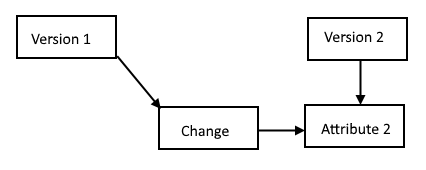
\includegraphics{figures/Addition.png}
	\begin{tikzpicture}[every node/.style={draw, rectangle}]
	\begin{scope}[node distance=10mm and 30mm]
	\node (1) [scale=1.25] at (0,0) {Version 1};
	\node (a) [below=of 1, scale=1.25] {Attribute};
	\node (p1) [below=of a, scale=1.25] {Pre-Value};
	\node (p2) [below right=of a, scale=1.25] {Post-Value};
	\node (n) [above=of p2, scale=1.25] {New};
	\node (o) [right=of n, scale=1.25] {Old};
	\node (2) [above =of o, scale=1.25] {Version 2};
	
	\draw [line width=2pt, ->] (1) -- (2);
	\draw [line width=2pt, ->] (2) -- (n);
	\draw [line width=2pt, ->] (2) -- (o);
	\draw [line width=2pt, ->] (1) -- (a);
	\draw [line width=2pt, ->] (2) -- (a);
	\draw [line width=2pt, ->] (a) -- (p1);
	\draw [line width=2pt, ->] (a) -- (p2);
	\end{scope}
	\end{tikzpicture}
	\caption{Provenance based versioning model.}
	\label{DiscardedFig}  % the \label command comes AFTER the caption
\end{figure}
Until the introduction of or comparison with Version 2, none of the concepts in Version 1 can be considered new or old.
As the responsible party for introducing changes, Version 2 becomes associated with \textit{New}, \textit{Old}, and modified attributes.
Version 1 also has a link to altered \glspl{attribute} since it provides the \textit{pre-value} used to contextualize Version 2's \textit{post-value}.
The pre- and post- values are included so that a user can see how much the \gls{attribute} has changed, much like with a \gls{log}.

Adding the \glspl{attribute} as concepts to the provenance based model addresses PROV's and PAV's flat approach to \gls{version} relations, but the \glspl{attribute} do not capture the inter-relation between objects for \textit{New} and \textit{Old} \glspl{attribute}.
Having Version 2 be responsible for all the changes causes issues with the model since it must be associated with \glspl{attribute} from an entirely different object.
The \textit{Old} \glspl{attribute} do not appear within Version 2, failing to meet the version-attribute connectivity requirement.
Associating \textit{Old} \glspl{attribute} with Version 1 would be more appropriate and intuitive to understand.
To test whether the provenance based model satisfied version continuity, a hypothetical third version is added.
For attributes which are modified in Versions 1, 2, and 3, all pre- and post-values are grouped under the singlar Attribute, making the sequence of values ambiguous.
Because the provenance based model cannot unambiguously accommodate a third version, version continuity is not upheld.

Using change logs as a basis, a log based model, shown in Figure \ref{DiscardedFig2} was created.
\begin{figure}
	\centering
	\vspace{0.0in} % normally the command here would be \includegraphics
	%	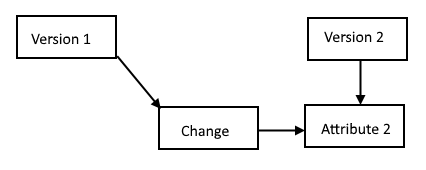
\includegraphics{figures/Addition.png}
	\begin{tikzpicture}[every node/.style={draw, rectangle}]
	\begin{scope}[node distance=10mm and 20mm]
	\node (l) [scale=1.25] at (1,0) {Log};
	\node (n) [above right=of l, scale=1.25] {New};
	\node (o) [below right=of l, scale=1.25] {Old};	
	\node (a) [right=of l, scale=1.25] {Attribute};
	\node (c) [right=of a, scale=1.25] {Change};
	\node (t) [right=of c, scale=1.25] {Type};
	\node (p1) [above right=of c, scale=1.25] {Pre-Value};
	\node (p2) [below right=of c, scale=1.25] {Post-Value};
	
	\draw [line width=2pt,->] (l) -- (n);
	\draw [line width=2pt,->] (l) -- (o);
	\draw [line width=2pt,->] (l) -- (a);
	\draw [line width=2pt,->] (a) -- (c);
	\draw [line width=2pt, ->] (c) -- (t);
	\draw [line width=2pt, ->] (c) -- (p1);
	\draw [line width=2pt, ->] (c) -- (p2);
	\end{scope}
	\end{tikzpicture}
	\caption{Change log based versioning model.}
	\label{DiscardedFig2}  % the \label command comes AFTER the caption
\end{figure}
\Glspl{attribute} are attached to the log as the primary indicators for old, new, and modified concepts.
\Glspl{log} often show a break down and group changes by \glspl{attribute}.
For modified \glspl{attribute}, an additional change concept is associated, encapsulating the values and nature of the change.
At the far right side of the figure is a concept called \textit{Type} which indicates more specifically the nature of the change, for example one unit of speed to another.
Pre- and post- values were also included to explicitly define the change concept.

The primary drawback of the log based model is that the Log concept is the origin for every modification to the data even though the document only reports the differences.
The \gls{version} objects are also left out of the log based model, leaving the Log concept in possession of the attributes.
One of the major breakthroughs with the log based model formulation is that while specific values are kept in the log, pre- and post- values do not need to be in a versioning model.
By encoding the type of change, the need for actual values becomes superfluous as change type is more generalizable across domains and contexts.

Figure \ref{DiscardedFig3} combines the provenance and change log approaches, resulting in the hybrid model, by modeling the change log as a transition between Version 1 and Version 2.
\begin{figure}
	\centering
	\vspace{0.0in} % normally the command here would be \includegraphics
	%	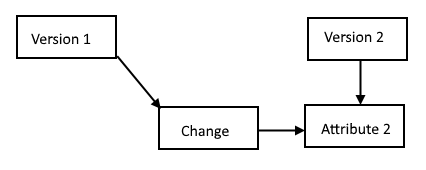
\includegraphics{figures/Addition.png}
	\begin{tikzpicture}[every node/.style={draw, rectangle}]
	\begin{scope}[node distance=10mm and 30mm]
	\node (l) [scale=1.25] at (0,0) {Log};
	\node (1) [left=of l, scale=1.25] {Version 1};
	\node (2) [right=of l, scale=1.25] {Version 2};
	\node (n) [below=of 1, scale=1.25] {New};
	\node (o) [below=of 2, scale=1.25] {Old};	
	\node (m) [below=of l, scale=1.25] {Modified};
	\node (a) [below=of m, scale=1.25] {Attribute};
	
	\draw [line width=2pt,->] (1) -- (l);
	\draw [line width=2pt,->] (l) -- (2);
	\draw [line width=2pt,->] (l) -- (m);
	\draw [line width=2pt,->] (l) -- (n);
	\draw [line width=2pt, ->] (l) -- (o);
	\draw [line width=2pt, ->] (m) -- (a);
	\end{scope}
	\end{tikzpicture}
	\caption{Hybrid provenance and change log versioning model.}
	\label{DiscardedFig3}  % the \label command comes AFTER the caption
\end{figure}
The idea enables distance capture between versions by encapsulating all changes within the Log concept.
The changes are then associated with specific \glspl{attribute}.
Pre- and post- values do not appear in the model because, as explained previously, the presence and kind of change is more valuable information than assessing the explicit values involved.
As the number of changing entries increases, more values would need to be stored, resulting in the copying of the data rather than summarization of the changes.
Notice in Figure \ref{DiscardedFig3} that \textit{Attribute} has now become disconnected from either Version concept.
Reconnecting the \textit{Attribute} concept brings into question which \gls{version} it should be associated with since it exists in both.
The larger issue with both the log based model and hybrid model is that the versioning model resembles a tree more than a graph, making \gls{linked} queries less powerful, as most of the concepts are disconnected.

A fourth formulation, in Figure \ref{DiscardedFig4}, leverages the insight that when a \textbf{change} interacts with an \gls{attribute}, the \gls{attribute} has changed in the next \gls{version}, resulting in the model referred to as the fully connected model.
\begin{figure}[b]
	\centering
	\vspace{0.0in} % normally the command here would be \includegraphics
	%	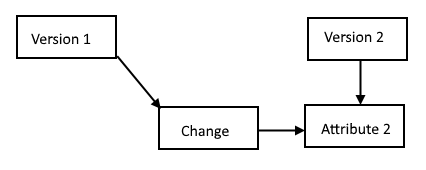
\includegraphics{figures/Addition.png}
	\begin{tikzpicture}[every node/.style={draw, rectangle}]
	\begin{scope}[node distance=20mm and 20mm]
	\node (c) [scale=1.25] at (1,0) {Change};
	\node (1) [above left=of c, scale=1.25] {Version 1};
	\node (2) [above right=of c, scale=1.25] {Version 2};
	\node (a1) [below =of 1, scale=1.25] {Attribute 1};
	\node (a2) [below =of 2, scale=1.25] {Attribute 2};
	
	\draw [line width=2pt,->] (a1) -- (c);
	\draw [line width=2pt,->] (a2) -- (c);
	\draw [line width=2pt, ->] (1) -- (a1);
	\draw [line width=2pt, ->] (2) -- (a2);
	\draw [line width=2pt,->] (c) -- (1);
	\draw [line width=2pt,->] (c) -- (2);
	\end{scope}
	\end{tikzpicture}
	\caption{Highly connected model of just versions, changes, and attributes}
	\label{DiscardedFig4}  % the \label command comes AFTER the caption
\end{figure}
The fully connected model addresses the attribution problem by forming two \glspl{attribute}, each associated with a different \gls{version}.
These \glspl{attribute} inform a \textbf{change} which acts upon both \textit{Version} concepts.
The \textit{Log} object is dropped for the fully connected model since it is a method to convey change and not an actor involved in the change.
The highly connected model is not able to capture new and old \textit{Attributes} because Attribute 1 and Attribute 2 cannot be removed from the model, meaning that the fully connected model cannot represent all additions, invalidations, and modifications.

One observation is that the relation from changes to \glspl{version} is redundant since the links from \textit{Version} to \textit{Attribute} to \textit{Change} implies the same relationship.
Removing the explicit relation would shorten the number of triples required to encode a change and improve scalability.
The \gls{vergraph} using the highly connected model would also be easier to query if the edges were oriented in the same direction, additionally implying that change flows from one \gls{version} to the next.
These final observations result in the final versioning model which is used to instantiate VersOn.

\section{The Final Model} \label{sec:model}

The final versioning model incorporates three kinds of objects: \glspl{version}, \glspl{attribute}, and \gls{change}.
A \gls{version} object represents the items being compared such as a book or spreadsheet.
In \gls{prov}, a \gls{version} would likely correspond with the \textit{prov:Entity} involved in a \textit{prov:wasRevisionOf} property.
The \textbf{attribute} object refers to specific parts which make up a \gls{version}.
\Glspl{attribute} could be lines in a book or columns in a spreadsheet.
Including \glspl{attribute} addresses the lack of detail involved in a \textit{prov:wasRevisionOf} or \textit{pav:previousVersion}.
The relationship between \textbf{versions} and \textbf{attributes} captures the influence that changes in the underlying part will have on the overarching \gls{version}.
Because the model refers to specific parts of a \gls{version}, the \gls{version} concept corresponds most closely with a \gls{frbr} \textbf{manifestation} rather than an \textbf{expression}.
The presence or absence of an \gls{attribute} is used to determine the kind of \gls{change} which occurs to the \gls{attribute} between \glspl{version}.
\Gls{change} are used to link together \glspl{attribute} from different \glspl{version}.
The \gls{change} captures a difference between the old \gls{version} state and the new \gls{version} state.
While the \gls{change} object greatly resembles a \gls{prov} qualified property, its form can change depending on the kind of \gls{change}, like a \textit{schema:UpdateAction}.
The final model is implemented by The Versioning Ontology (VersOn).
The full ontology map can be seen in Figure \ref{vo_map}.
\begin{figure}
	\centering
	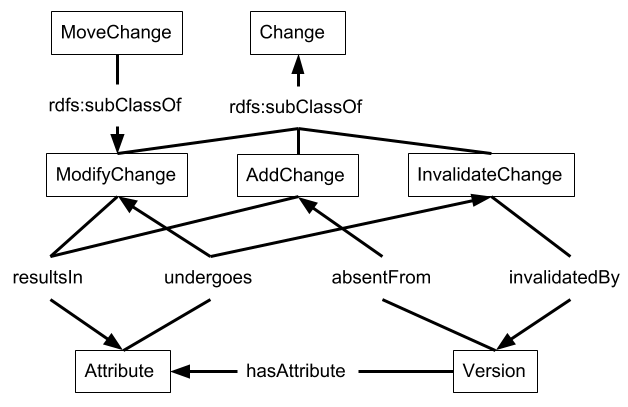
\includegraphics[scale=.9]{figures/OntologyMap.png}
	\caption{Ontology map of the Versioning Ontology.  The primary concepts are Version, Attribute, and Change.  Changes are subclassed into disjoint AddChange, InvalidateChange, and ModifyChange concepts.  The MoveChange is a subclass of ModifyChange, demonstrating the extension of the core change concepts.}
	\label{vo_map}
\end{figure}

\subsection{Left-hand Right-hand Convention}

In the following diagrams and figures, the original or base \gls{version} and its \glspl{attribute} will be placed on the left-hand side and the new \gls{version} will be placed on the right-hand side with its \glspl{attribute}.
References to the \glspl{version} as previous and next are avoided since sequencing may not play a major role in distinguishing \glspl{version}.
Scientific data in large repositories often track sequential releases of data, but a book may have different \glspl{version} distinguished by printed language.
To recognize the distinction, objects will be referred to as the \textbf{left-hand version} or \textbf{left-hand attribute} when they are not sequentially or temporally related.

\section{How Changes are Represented in the Model}

The final model bases \glspl{change} around the three core versioning operations because their commonality across systems provides a fundamental basis for comparisons.
\glspl{add} occur when an \gls{attribute} appears only in the \textbf{right-hand version}.
When an \gls{attribute} only shows up in the \textbf{left-hand version}, the final model captures the relationship as an \gls{invalidate}.
Finally, a \gls{modify} change has \glspl{attribute} in both the \textbf{left-} and \textbf{right-hand versions}, but the \gls{modify} change only connects two \glspl{attribute} if the values are different.
These three combinations cover the possible situations within the final model.

\begin{figure}
	\centering
	\vspace{0.0in} % normally the command here would be \includegraphics
	%	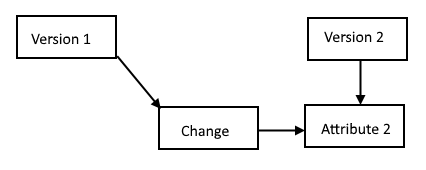
\includegraphics{figures/Addition.png}
	\begin{tikzpicture}[every node/.style={draw, rectangle}]
	\begin{scope}[node distance=20mm and 20mm]
	\node (c) [scale=1.25] at (1,0) {Change M};
	\node (1) [above left=of c, scale=1.25] {Version 1};
	\node (2) [above right=of c, scale=1.25] {Version 2};
	\node (a1) [below =of 1, scale=1.25] {Attribute 1};
	\node (a2) [below =of 2, scale=1.25] {Attribute 2};
	
	\draw [line width=2pt,->] (a1) -- (c);
	\draw [line width=2pt,->] (c) -- (a2);
	\draw [line width=2pt, ->] (1) -- (a1);
	\draw [line width=2pt, ->] (2) -- (a2);
	\end{scope}
	\end{tikzpicture}
	\caption{Model of the relationships between Versions 1 and 2 when modifying Attribute 1 from Version 1 as a result of Change M, resulting in Attribute 2 from Version 2}
	\label{ModificationFig}  % the \label command comes AFTER the caption
\end{figure}

\subsection{Modification}

The \gls{modify} relation occurs when an \gls{attribute} appears in both \glspl{version} and their values are different.
In Figure \ref{ModificationFig}, a \gls{modify} is captured between two \glspl{version}.
Each \gls{version} has an \gls{attribute}, Attribute 1 and Attribute 2, respectively.
Finally, a \gls{change} object connects the two \glspl{attribute}, denoting that the values described by the \gls{attribute} are different.

The specific values pertaining to Attribute 1 and Attribute 2 are not captured by the model because acknowledging that a difference exists is more important.
Extending the model to properly communicate the significance of a modification for a wide variety of domains would require sizable domain knowledge and would be outside of a data versioning scientist's domain.
In addition, the model would essentially begin storing a copy of the data set, leading to space and redundancy concerns.

In some applications, a \textbf{modification} is represented as an \textbf{invalidation} followed by an \textbf{addition}.
The representation has a couple of problems.
The first is that the sequence of changes implies that there is an intermediary stage where all the modified values have been invalidated but not added.
The intermediary stage constitutes a new version of the data object, even though only one change is being made.
The second issue with using the two change sequence is that the two states of attribute, before and after the \textbf{modification}, becomes disassociated.
Any new attribute being added to the version is not necessarily associated with an attribute in the left-handed version.
Establishing the association between attributes after an \textbf{invalidation}-\textbf{addition} sequence is the same as and more concisely expressed as a \textbf{modification}.

\subsection{Addition}

In Figure \ref{AdditionFig}, the \gls{add} model differs from the \gls{modify} construction by the absence of Attribute 1.
\begin{figure}
	\centering
	\vspace{0.0in} % normally the command here would be \includegraphics
	%	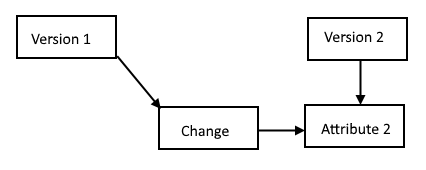
\includegraphics{figures/Addition.png}
	\begin{tikzpicture}[every node/.style={draw, rectangle}]
	\begin{scope}[node distance=20mm and 20mm]
	\node (c) [scale=1.25] at (1,0) {Change A};
	\node (1) [above left=of c, scale=1.25] {Version 1};
	\node (2) [above right=of c, scale=1.25] {Version 2};
	\node (a) [below =of 2, scale=1.25] {Attribute 2};
	
	\draw [line width=2pt,->] (1) -- (c);
	\draw [line width=2pt,->] (c) -- (a);
	\draw [line width=2pt, ->] (2) -- (a);
	\end{scope}
	\end{tikzpicture}
	\caption{Model of the relationships between Versions 1 and 2 when adding an Attribute 2 to Version 2 as a result of Change A}
	\label{AdditionFig}  % the \label command comes AFTER the caption
\end{figure}
The absence creates a disconnect between ``Version 1" and ``Change A".
We know that a connected graph will be desirable to accommodate traversal using \gls{linked} query languages so ``Version 1" must be reconnected to the other concepts in the model.
A \textbf{property} is used to create a path between the two \glspl{attribute} to indicate the contribution of  ``Version 1" to the \gls{change}'s \gls{provenance}.
The path does not show that ``Version 1" informs or creates ``Attribute 2", while that may be true.
The construction was also chosen to create a symmetric orientation with the \gls{invalidate} change.


\subsection{Invalidation}

The \gls{invalidate} model has a missing \gls{attribute} on the right-hand side of the relation, contrary to the \gls{add} construction.
As a result of the invalidation, an \gls{attribute} no longer exists in the \textbf{right-hand version}.
As seen in Figure \ref{InvalidationFig}, the \gls{invalidate} change concept matches to the Version 2 object.
\begin{figure}
	\centering
	\vspace{0.0in} % normally the command here would be \includegraphics
	%	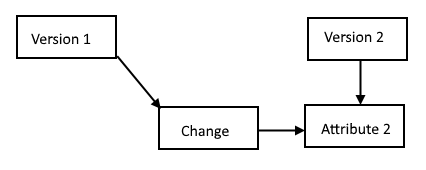
\includegraphics{figures/Addition.png}
	\begin{tikzpicture}[every node/.style={draw, rectangle}]
	\begin{scope}[node distance=15mm and 20mm]
	\node (c) [scale=1.25] at (1,0) {Change I};
	\node (1) [above left=of c, scale=1.25] {Version 1};
	\node (2) [above right=of c, scale=1.25] {Version 2};
	\node (a) [below =of 1, scale=1.25] {Attribute 1};
	
	\draw [line width=2pt,->] (a) -- (c);
	\draw [line width=2pt,->] (c) -- (2);
	\draw [line width=2pt, ->] (1) -- (a);
	\end{scope}
	\end{tikzpicture}
	\caption{Model of the relationships between Versions 1 and 2 when invalidating Attribute 1 from Version 1 as a result of Change I}
	\label{InvalidationFig}  % the \label command comes AFTER the caption
\end{figure}
Just like in the \gls{add} model, the \gls{invalidate} construction maintains a link between the two \gls{version} objects.
In the \gls{invalidate} case, it makes more conceptual sense, however, because ``Version 2" invalidates ``Attribute 1" by omitting the \gls{attribute}.


\section{Utilized Data Sets}

\subsection{Noble Gas Data set}

The ``Global Database on \textsuperscript{3}He/\textsuperscript{4}He in on-shore free-circulated subsurface fluids" is a tumultuous database \cite{Polyak2015}.
The first \gls{version}, published in June 11, 2013, contains the information from 8 regions of the world united into a single file with 199 columns.
The next \gls{version} of the database, published March 8, 2015, reduces the number of columns to 54, marking a drastic change.
In addition, several columns changed the units with which they reported measurements.
While usage documentation, explaining the content and use of the data, accompanied each \gls{version}, no records were included indicating what changed between \glspl{version}.
A \gls{log} would be valuable guide with such drastic structural and content changes.
The third and most recent publication came in July 11, 2017, with no changes to the number of files or columns, but many new rows.
The structural summary of each of the files can be found in Table \ref{noble_gas_file_table}.

\begin{table}
	\caption{Files in the Noble Gas data set.}
	\label{noble_gas_file_table}
	\centering
	\begin{tabular}{|c|c|c|c|c|}
		\hline
		Filename & File Size (Bytes) & Rows & Columns &	Total Cells \\ \hline
		DB\_HE\_6733.xlsx &	2682683 &	6733 &	199 &	1339867 \\
		DB\_final-55-7262\_2015\_03 &	2729060 &	7265 &	54 &	392310 \\
		\_08.xlsx&&&&\\
		NG\_DB\_final\_2017\_07 &	4216595 &	8231 &	54 &	444474 \\
		\_01.xlsx&&&&\\
		\hline
	\end{tabular}
\end{table}

\subsection{Copper Data set}

The Paragenetic Mode for Copper Minerals database became available through collaboration with the author's lab to create new methods of visualizing mineralogy relationships \cite{Morrison2016}.
The first version was collected June 8, 2016, with the update following soon after on August 8, 2016.
Major edits are fairly limited with only 16 column additions and 2 removals between the versions.
Value formats remain consistent from one version to the next, resulting in a much more condensed body of changes, making transitions more easily verifiable.
Compared to the Noble Gas data set, it provides a more stable data platform to implement the versioning model in Section \ref{sec:model}.
The data from Copper Minerals is also more processing friendly, making it agreeable to automatic \gls{log} generation.
An interesting thing to note in Table \ref{copper_file_table} is that the second version takes up less storage space even though it has more data.

\begin{table}
	\caption{Files in the Copper data set.}
	\label{copper_file_table}
	\centering
	\begin{tabular}{|c|c|c|c|c|}
		\hline
		Filename & File Size (Bytes) & Rows & Columns &	Total Cells \\ \hline
		ParageneticModeTable\_Cu\_6. &	339175 & 705 &	37 &	26085\\
		8.2016.xlsx&&&&\\
		ParageneticModeTable\_Cu\_8. & 233715 & 685 & 51 & 34935\\
		21.2016.xlsx&&&&\\
		\hline
	\end{tabular}
\end{table}

\section{Summary}

The versioning model provides a method to capture \gls{change} information in greater detail than current provenance models.
The inclusion of \glspl{version} and \glspl{attribute} into the model connect changing items with the objects they influence.
The \glspl{change} create a ladder-like structure to connect \gls{version} objects in greater detail.
Each rung of the ladder can not only be counted, but also grouped into types of change according to the respective operation.
The method of instantiating a \gls{vergraph} will be covered in Chapter \ref{ch:graph}.

